\section{Härten von mobilen Anwendungen}
	Trotz aller vorhandenen Hilfsmittel sollte man nicht allein auf die Sicherheit
	von iOS vertrauen. Deshalb listet der Author abschließend je ein Unterkapitel
	für Entwickler und für Endnutzer, in welchen mögliche Verbesserungen für die
	Entwicklung einer App oder für das Einrichten von iOS Geräten aufgezeigt
	werden.
	\subsection{Relevantes für den Entwickler}
		Der Entwickler ist verantwortlich für die Sicherheit seiner Anwendung und
		sollte jegliche mögliche Option der zusätzlichen Absicherung seiner
		Applikation in Erwägung ziehen. Die folgenden Unterkapitel stellen eine
		Auflistung der wichtigsten Maßnahmen zum Schutz der eigens entwickelten App
		dar. An dieser Stelle gilt es zu erwähnen, dass es sich hier nicht um nicht
		alle Möglichkeiten handelt und vor allem, dass keine Applikation absolut
		sicher gemacht werden kann. Aber zieht man die folgenden Herangehensweisen in
		Betracht, kann dies die Sicherheit einer App steigern und die
		Zeit enorm erhöhen, welche für einen erfolgreichen Angriff nötig ist.
		\subsubsection{Passwortstärke}
			Die Verschlüsselung ist eine der wichtigsten Arten seine Daten zu schützen,
			aber auch die kritischste, wenn es um die Implementierung geht. Daher richten
			Hacker ihr Augenmerk zuerst auf die Implementierung und nicht die
			eigentlichen verschlüsselten Daten. Hierbei ist es besonders wichtig, keine
			schwachen Passwörter zu erlauben. Eine strenge Passwortrichtlinie ist
			Pflicht, auch wenn es die Useability negativ beeinflusst. Die gewählten
			Passwörter sollten aus vielen Stellen bestehen (mindestens 12),
			welche wiederrum zu einem Anteil aus Zahlen, Sonderzeichen und Zeichen, in
			Groß- und Kleinschreibweise, bestehen. Zusätzlich sollten bestimmte Muster,
			wie entlang der QUERTZ-Tastatur zu fahren, einfache Wörter, welche meist in
			Dictionaries enthalten sind und strukturierte Daten wie ein Datum, verhindert
			werden.
		\subsubsection{Common Crypto Library}\label{sec:3cc}
			IOS bietet mit der \textsl{Common Crypto Library}\cite{3CC2007}
			(3CC oder auch CCCrypt) eine Möglichkeit auf C-Ebene 
			Verschlüsselungsalgorithmen wie AES, DES oder 3DES einzusetzen. Dabei bietet
			3CC je nach eingesetztem Algorithmus Block- beziehungsweise Stromchiffre an.
			Zusätzlich wird mit dem \textsl{Cipher Block Chaining} eine
			Möglichkeit angeboten, um Man-In-The-Middle, sowie Replay-Angriffe zu
			verhindern. Dies ist möglich, da bei CBC\footnote{CBC: Cipher Block Chaining}
			jeder Klartext-Block mit dem vorherigen verschlüsselten Chiffre
			XOR-verknüpft wird und anschließend ebenfalls chiffriert wird. Somit ist
			jeder Block von der bisherigen Kette verschlüsselter Daten abhängig.
		\subsubsection{Sicherung des Hauptschlüssels}\label{sec:master-key}		
			Falls ein Master-Key - also ein übergeordneter Schlüssel - zur
			Verschlüsselung eingesetzt wird, sollte dieser zwingend ebenso verschlüsselt
			werden. Das National Institute of Standards and Technology
			empfiehlt\cite{NISTPBKDF2010} dazu Passwort basierte 
			Schlüsselableitungsfunktionen (Password-Based Key Derivation Function),
			allgemein unter dem Kürzel \textsl{PBKDF2} bekannt.
			Diese leiten die Eingabe über mehrere, beziehungsweise eine gewünschte Anzahl
			von Iterationen zu einem Schlüssel der gewünschten Komplexität ab. Dieses
			Ergebnis wird dann genutzt, um den Master-Key zu verschlüsseln. Der
			eigentliche Vorteil bei dieser Herangehensweise liegt darin, dass der
			Master-Key nie geändert werden muss. Wenn der Nutzer beispielsweise sein
			Passwort ändert, muss der Master-Key nur mit dem neuen Passwort abgeleitet
			über die PBKDF verschlüsselt werden. Außerdem ist es bei diesem Ansatz
			möglich mehrere Kopien des Hauptschlüssel auf verschiedenen Wegen
			abzuspeichern. Ein Anwendungsbeispiel stellt die
			Verwendung von Rücksetzungsmechanismen von Passwörtern dar, wobei der
			Benutzer aufgefordert wird die Antwort auf eine bestimmte Frage zu geben,
			welche er zur Erstellung des Passwortes festgelegt hat. Hier wird der
			Master-Key also einmal mit der Passphrase des Nutzers verschlüsselt und
			einmal mit der Antwort der Sicherheitsfrage.
		\subsubsection{Lokations- und Tempusberücksichtigung}
			Sogenannte Geo-Encryption bringt einen weiteren Faktor in die Kette der
			möglichen Verbesserungen des Schutzes für unsere Applikation. Damit wird
			ein gewisser Aufenthaltsort, oder ein Radius um diesen vorgeschrieben. Das
			Gerät muss sich in diesem befinden, um eine Entschlüsselung zu ermöglichen.
			Zusätzlich kann die Zeit immer eine weitere Optimierung sein, indem die
			Entschlüsselung nur in einem gewissen Zeitfenster erlaubt wird.
		\subsubsection{Bipartite Schlüssel}
			Diese Vorgehensweise stellt eine - ähnlich zur Geo-Verschlüsselung - zweite
			Abhängigkeit im Entschlüsselungsprozess dar. Hierbei werden zwei Schlüssel
			beim erstmaligen Start der Applikation erzeugt und mit einander
			XOR-verknüpft. Dieses Ergebnis wird dann zum Verschlüsseln des
			Hauptschlüssels (Kapitel \ref{sec:master-key}) verwendet. Einen Anteil des
			Schlüssels stellt die Passphrase des Nutzers dar. Die andere ein
			erzeugter Zufallswert, welcher an einen entfernten Authorisierungsserver
			geschickt wird. Beim Start der App muss sich der Benutzer sowohl durch seine
			gewählte Passphrase lokal Authentifizieren, als auch beim Server anmelden,
			um den dort gespeicherten Zufallswert zu erhalten. Diese beiden Werte werden
			anschließend XOR-verknüpft, um damit den Master-Key zu entschlüsseln, mit
			welchem die Daten entschlüsselt werden. Falls ein Gerät als gestohlen
			vermutet wird, kann hier einfach der Serverseitige Schlüssel verworfen
			werden und jegliche Bemühungen des Angreifers, an die Daten zu kommen, wären
			vergebens.
		\subsubsection{Manipulationsschutz}
			Wenn ein Gerät gestohlen wurde, gibt es verschiedene Möglichkeiten den
			Schaden minimal zu halten und weiteren zu verhindern. Das Löschen von lokalen
			Benutzerdaten zählt zu diesen Maßnahmen. Dabei muss im Idealfall nur der
			Master-Key, welcher die relevanten Daten verschlüsselt,	überschrieben,
			beziehungsweise gelöscht werden und die Nutzerdaten sind unwiederherstellbar
			für den Angreifer(Vergleiche Kapitel \ref{sec:filesecurity}). Diese
			Herangehensweise ist unauffälliger, als beispielsweise ein komplettes
			"`Nullen"' der Datenbank und kostet den Angreifer frustrierende Zeit.\\
			Im Falle einer Manipulation muss davon ausgegangen werden, dass der Benutzer
			nicht mehr vertrauenswürdig ist. Somit sollte parallel zur Löschung der
			lokalen Daten eine eventuell vorhandene Anbindung an entfernte Resourcen
			(zum Beispiel Server, welche Daten für die App speichern) unterbrochen
			werden.	Dies kann bereits mit dem Setzen eines Flags in einer
			Konfigurationsdatei, oder dem Deaktivieren der Credentials des Nutzers auf
			Serverseite realisiert werden. Auf diese Weise handeln wir präventiv gegen
			weitere Schäden, ohne dass der Angreifer davon etwas erfährt.
		\subsubsection{Jailbreakerkennung}
			Es kann erwünscht sein, dass die entwickelte App nicht auf
			jailbroken\footnote{Jailbroken: bezeichnet Geräte auf denen ein Jailbreak
			installiert ist} iOS Geräten installiert werden darf.
			Da man sich bei diesen Geräten nicht mehr auf den nativen von iOS gegebenen Schutz (Kapitel
			\ref{sec:components-syssec}) verlassen kann (Kapitel \ref{sec:jailbreaking}).
			Diese Erkennung wird über einen Integritätstest der Sandbox mit dem
			Ausführen des Befehls \textsl{fork} getestet\cite[S.328]{Zdziarski2012}.
			Dieser erlaubt der App einen Kinds-Prozess zu starten. Wenn die Sandbox
			kompromittiert wurde, oder die App außerhalb dieser läuft, wird die
			Operation erfolgreich ausgeführt. Folgender Programmcodeauszug zeigt
			besagten Vorgang:
			\lstdefinestyle{customc}{
				belowcaptionskip=1\baselineskip,
			  	breaklines=true,
			  	frame=L,
			  	xleftmargin=\parindent,
			  	language=C,
			  	showstringspaces=false,
			  	basicstyle=\footnotesize\ttfamily,
			  	keywordstyle=\bfseries\color{green!40!black},
			  	commentstyle=\itshape\color{purple!40!black},
			  	identifierstyle=\color{blue},
			  	stringstyle=\color{orange},
			}
			\lstinputlisting[language=C]{ios/code/jailbreakdetection.c}
			
	\subsection{Tips für den Benutzer}
		Als Endnutzer hat man ebenfalls eine gewisse Fülle an Möglichkeiten seine
		Daten zu schützen und bedächtig vorzugehen. Dies bezieht sich in diesem Fall
		aber auf die Ebene des User Interfaces und dessen Einstellungen.
		\subsubsection{Lockscreen einschränken}
			In früheren iOS Versionen gab es bereits mehrere Male die Möglichkeit den
			gesperrten Bildschirm des Gerätes zu umgehen
			\cite{IOS7LockscreenBypass2013}.
			Dies kann verhindert werden, indem dafür nötige Dienste - zumindest für den
			Lockscreen - deaktiviert werden. Wenn die Sprachsteuerung \textsl{Siri} nicht benötigt
			wird, sollte diese ebenfalls für den Sperrbildschirm deaktiviert werden.
			Generell gilt hier ein Weniger-ist-Besser-Vorgehen.
		\subsubsection{Zwei-Faktor-Authentifizierung }
			Zu einem der wichtigsten sicherungssteigernden Möglichkeit von iOS Nutzern
			gehört die Zwei-Faktor-Authentifizierung. Diese fordert den Nutzer - sofern
			aktiviert - dazu auf, beim Einloggen in seinen Apple ID Account von einem
			bisher unbekannten Browser oder Gerät, einen Verifizierungsschlüssel
			einzugeben, der auf seinen restlichen iOS Geräten angezeigt
			wird\cite{AppleiOS9Preview2015}.
		\subsubsection{Privacy}
			Ab iOS 8 muss der Entwickler in seiner App hinterlegen, warum diese ein
			bestimmtes Recht, wie zum Beispiel Lokalisierungsdienste, erhalten will.
			Dieser Dialog erscheint, sobald die App dieses Recht erfragt und wird für den
			Nutzer sichtbar als Dialogbox mit Wahloptionen angezeigt.
			\begin{figure}[h]
				\centering
				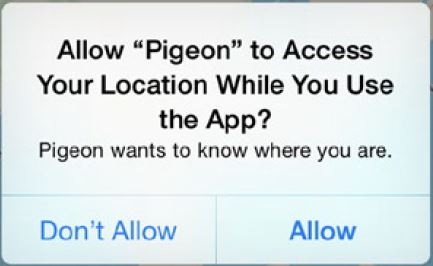
\includegraphics[width=0.4\linewidth]{ios/media/privacy-dialog.jpg}
				\caption{Authorisierungsdialog für den Aufenthaltsort 
				\cite[S.535]{LearnIOS7Dev2013}}
				\label{fig:privacy-dialog}
			\end{figure}
			Sobald dieser Dialog durch eine Auswahl verschwindet, kann man diese
			Einstellung auch unter den Systemeinstellungen finden. Dazu öffnet man diese
			und wählt danach den Punkt "`Privacy"'. Unter dieser Auswahl werden alle Apps
			angezeigt, die den Lokalisierungsdienst nutzen. So hat der Nutzer zu jeder
			Zeit die Möglichkeit die Einstellungen zu ändern und es nach Belieben
			anzupassen. Außerdem ist es möglich diese Regeln jeweils für
			Kontakte, Kalender, Erinnerungen, Fotos, Bluetooth, Mikrophon, Kamera,
			HealthKit, HomeKit und Motion Activity individuell einzustellen. Zusätzlich
			gibt es noch Einstellungen für die sozialen Netzwerke Facebook und Twitter.
			%TODO: put screenshot into this section
			Zuletzt kann man das Advertising gezielt beeinflussen, indem man es über
			"`Limit Ad Tracking"' setzt. Über diese Einstellung wird gezielt Werbung für
			den Nutzer aufgrund dessen Verhalten generiert und dann in entsprechenden
			Umgebungen (Webseiten oder Apps mit Werbung) angezeigt. Hier muss erwähnt
			werden, dass diese Einstellung auf Browserseite nur bei dem unter iOS
			vorinstallierten Safari wirkt. Alle anderen ignorieren diese Einstellung.
			\cite{AppleMngPrivacy2015}\cite[S.131]{IKungFu2014}.
		\subsubsection{Periodisches Ändern des Passwortes der Apple-ID}
			Durch ein regelmäßiges Ändern des Passwortes der Apple-ID wird verhindert,
			dass ein Passwort das in die falschen Hände gelangte, lange von Nutzen ist.
			Der Author empfiehlt dieses Vorgehen nicht nur auf iOS zu beschränken.
			Generell ist es empfehlenswert dies bei allen Passwörtern anzuwenden.
